\chapter[Models]{Physical and numerical models}

\section{Physical and mathematical description} 

Characteristic of compositional multiphase models is that the phases
are not only matter of a single chemical substance. Instead, their
composition in general includes several species, and for the mass transfer, 
the component behavior is quite different from the phase behavior. In the following, we
give some basic definitions and assumptions that are required for the
formulation of the model concept below. As an example, we take a
three-phase three-component system water-NAPL-gas
\cite{A3:class:2002a}. The modification for other multicomponent
systems is straightforward and can be found, e.\ g., in
\cite{A3:bielinski:2006,A3:acosta:2006}.

\subsection{Basic Definitions and Assumptions for the Compositional
  Model Concept}
\textbf{Components:}
The term {\it component} stands for constituents of the phases which
can be associated with a unique chemical species, or, more generally, with 
a group of species exploiting similar physical behavior. In this work, we
assume a water-gas-NAPL system composed of the phases water (subscript
$\text{w}$), gas ($\text{g}$), and NAPL ($\text{n}$). These phases are
composed of the components water (superscript $\text{w}$), air
($\text{a}$), and the organic contaminant ($\text{c}$) (see Fig.\
\ref{fig:phaseMassEnergyTransfer}).

\begin{figure}
  \centering
  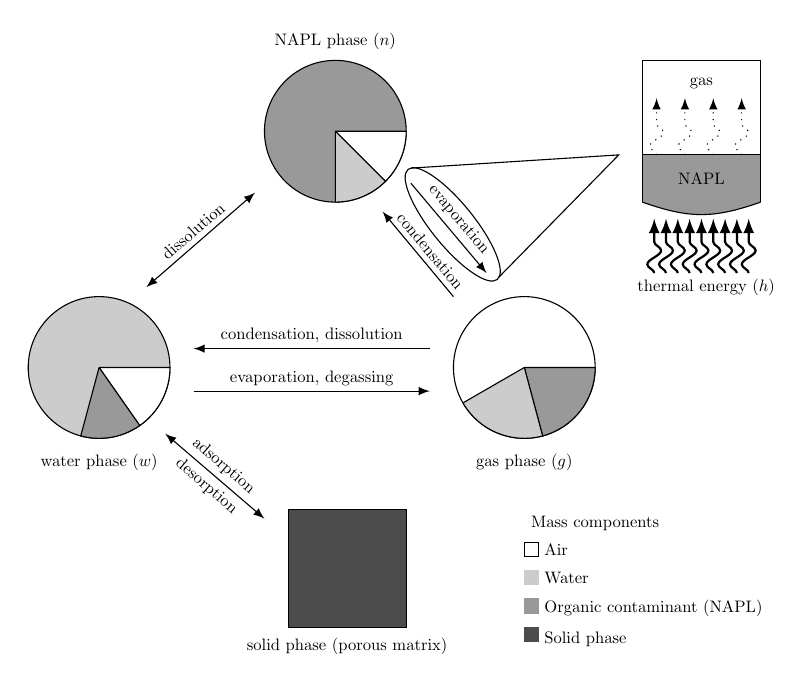
\begin{tikzpicture} [>=latex,scale=0.6, every node/.style={transform shape}]
    % Ellipse 1 solid
    \coordinate (A) at (1,-0.5);
    \draw [fill=black!70](A) rectangle(3.5,2) node at(2.25,-0.9) {solid phase (porous matrix)};
    % Ellipse 2 water
    \coordinate (B) at (-3,5);
    \draw [fill=black!20](B) circle(1.5cm);
    \node [yshift=5mm]at(-3,2.5){water phase $(w)$};
    \draw[fill=white] (B)--+(1.5,0)arc(0:-55:1.5cm)--(B);
    \draw[fill=black!40] (B)--+(-55:1.5cm)arc(-55:-105:1.5cm)--(B);
    % Ellipse 3 gas
    \coordinate (C) at (6,5);
    \draw [](C) circle (1.5cm);
    \node[yshift=5mm]at(6,2.5){gas phase $(g)$};
    \draw [fill=black!40](C)--+(1.5,0)arc(0:-75:1.5cm)--(C);
    \draw [fill=black!20] (C)--+(-75:1.5cm)arc(-75:-150:1.5cm)--(C);
    % Ellipse 4 napl
    \coordinate (D) at (2,10);
    \draw [fill=black!40](D) circle (1.5cm);
    \node[yshift=5mm]at(2,11.4){NAPL phase $(n)$};
    \draw [fill=white](D)--+(1.5,0)arc(0:-45:1.5cm)--(D);
    \draw [fill=black!20] (D)--+(0,-1.5)arc(-90:-45:1.5cm)--(D);
    % arrows
    %A-B
      \draw [<->,white](0.5,1.8)--(-1.6,3.6) node[black,above,sloped,pos=0.5]{adsorption};
      \draw [<->](0.5,1.8)--(-1.6,3.6) node[below,sloped,pos=0.5]{desorption};
    %B-C 
      \draw[<-](-1,5.4)--(4,5.4)node[above,sloped,pos=0.5]{condensation, dissolution};
      \draw[->](-1,4.5)--(4,4.5)node[above,sloped,pos=0.5]{evaporation, degassing};
    %B-D
      \draw[<->](-2,6.7)--(0.3,8.7)node[above,sloped,pos=0.5]{dissolution};
    %D-C
      \draw[->](3.6,8.9)--(5.2,7)node[above,sloped,pos=0.5]{evaporation};
      \draw[rotate around={-51:(4,6.8)}](3.35,7.95) ellipse (1.5cm and 0.45cm);  %Ellipse um evaporation
      \draw (3.6,9.22)--(8,9.5)--(5.45,6.9); 
      \draw[<-](3,8.3)--(4.5,6.5)node[above,sloped,pos=0.55]{condensation};
    % thermal energy
    \filldraw [black!40](8.5,9.5)rectangle(11,8.5);
    \draw (8.5,9.5)rectangle(11,11.5);
    \draw (8.5,9.5)--(8.5,8.5);
    \draw (11,9.5)--(11,8.5);
    \draw [decorate,decoration={bent,aspect=0.4,amplitude=6},fill=black!40](11,8.5)--(8.5,8.5);
    \foreach \x in {8.75,9,...,10.8}
    \draw [->,decorate,decoration={snake,post length=2mm},thick](\x,7)--(\x,8.15);
    \foreach \x in {8.8,9.4,10,10.6}
    \draw [->,dotted,decorate,decoration={snake,post length=2mm}](\x,9.5)--(\x,10.7);
    \node at(9.75,11){gas};
    \node at(9.75,9){NAPL};
    \node at(9.85,6.7){thermal energy $(h)$};
    % legende
    \node at (7.5,1.7){Mass components};
    \draw[](6,1)rectangle +(0.3,0.3) node at(6.3,1.15) [right]{Air};
    \filldraw[black!20](6,0.4) rectangle +(0.3,0.3) node at (6.3,0.55)[black,right]{Water};
    \filldraw[black!40](6,-0.2) rectangle +(0.3,0.3) node at (6.3,-0.1)[right,black]{Organic contaminant (NAPL)};
    \filldraw[black!70](6,-0.8) rectangle +(0.3,0.3) node at (6.3,-0.75)[right,black]{Solid phase};
  \end{tikzpicture}
  \caption{Mass and energy transfer between the phases}
  \label{fig:phaseMassEnergyTransfer}
\end{figure}

\textbf{Equilibrium:}
For the non-isothermal multiphase processes in porous media under
consideration, we state that the assumption of local thermal
equilibrium is valid since flow velocities are small. We neglect
chemical reactions and biological decomposition and assume chemical
equilibrium.  Mechanical equilibrium is not valid in a porous medium, 
since discontinuities in pressure can occur across a fluid-fluid
interface due to capillary effects.

\textbf{Notation:} The index $\alpha \in \{\text{w}, \text{n}, \text{g}\}$ refers 
to the phase, while the superscript $\kappa \in \{\text{w}, \text{a}, \text{c}\}$ refers 
to the component. \\
\begin{tabular}{llll}
$p_\alpha$ & phase pressure & $\phi$ & porosity \\
$T$ & temperature & $K$ & absolute permeability tensor \\
$S_\alpha$ & phase saturation & $\tau$ & tortuosity \\
$x_\alpha^\kappa$ & mole fraction of component $\kappa$ in phase $\alpha$ & $\boldsymbol{g}$ & gravitational acceleration \\
$X_\alpha^\kappa$ & mass fraction of component $\kappa$ in phase $\alpha$ & $q^\kappa_\alpha$ & volume source term of $\kappa$ in $\alpha$ \\
$\varrho_{\text{mol},\alpha}$ & molar density of phase $\alpha$ & $u_\alpha$ & specific internal energy \\
$\varrho_{\alpha}$ & mass density of phase $\alpha$ & $h_\alpha$ & specific enthalpy \\
$M$ & molar mass of a phase or component & $c_\text{s}$ & specific heat enthalpy \\
$k_{\text{r}\alpha}$ & relative permeability & $\lambda_\text{pm}$ & heat conductivity \\
$\mu_\alpha$ & phase viscosity & $q^h$ & heat source term \\
$D_\alpha^\kappa$ & diffusivity of component $\kappa$ in phase $\alpha$ & $\boldsymbol{v}_{a,\alpha}$  & advective velocity \\
$\boldsymbol{v}_\alpha$ & Darcy velocity & & \\
\end{tabular}


\subsection{Balance Equations}
For the balance equations for multicomponent systems, it is in many
cases convenient to use a molar formulation of the continuity
equation. Considering the mass conservation for each component allows
us to drop source/sink terms for describing the mass transfer between
phases. Then, the
molar mass balance can be written as:
%
\begin{multline}
  \label{A3:eqmass1}
 \phi \frac{\partial (\sum_\alpha \varrho_{\text{mol}, \alpha}
    x_\alpha^\kappa S_\alpha )}{\partial t}  
 - \sum\limits_\alpha \Div \left\lbrace \frac{k_{\text{r}
        \alpha}}{\mu_\alpha} \varrho_{\text{mol}, \alpha}
    x_\alpha^\kappa \textbf{K} (\grad p_\alpha -
    \varrho_{\alpha} \boldsymbol{g}) \right\rbrace  \\
  % 
  %
 - \sum\limits_\alpha \Div \left\lbrace \tau \phi S_\alpha D_\alpha^\kappa \varrho_{\text{mol},
      \alpha} \grad x_\alpha^\kappa \right\rbrace
 - q^\kappa = 0, \qquad \kappa \in \{\text{w,a,c}\}.
\end{multline}

The component mass balance can also be written in terms of mass fractions 
by replacing molar densities by mass densities and mole by mass fractions.
To obtain a single conserved quantity in the temporal derivative, the total 
concentration, representing the mass of one component per unit volume, is defined as
\begin{displaymath}
C^\kappa = \sum_\alpha \phi S_\alpha \varrho_{\text{mass},\alpha} X_\alpha^\kappa \; .
\end{displaymath}
Using this definition, the component mass balance is written as:

\begin{multline}
  \label{A3:eqmass2}
    \frac{\partial C^\kappa}{\partial t} = 
  \sum\limits_\alpha \Div \left\lbrace \frac{k_{\text{r}
        \alpha}}{\mu_\alpha} \varrho_{\text{mass}, \alpha}
    X_\alpha^\kappa \textbf{K} (\grad p_\alpha +
    \varrho_{\text{mass}, \alpha} \boldsymbol{g}) \right\rbrace  \\
  %
  %
   + \sum\limits_\alpha \Div \left\lbrace \tau \phi S_\alpha D_\alpha^\kappa \varrho_{\text{mass},
      \alpha} \frac{M^\kappa}{M_\alpha} \grad x_\alpha^\kappa \right\rbrace 
 + q^\kappa = 0, \qquad \kappa \in \{\text{w,a,c}\}.
\end{multline}


In the case of non-isothermal systems, we further have to balance the
thermal energy. We assume fully reversible processes, such that entropy
is not needed as a model parameter. Furthermore, we neglect 
dissipative effects and the heat transport due to molecular
diffusion. The energy balance can then be
formulated as:
%
\begin{multline}
  \label{A3:eqenergmak1}
  \phi \frac{\partial \left( \sum_\alpha \varrho_{\alpha}
      u_\alpha S_\alpha \right)}{\partial t} + \left( 1 -
    \phi \right) \frac{\partial \varrho_{\text{s}} c_{\text{s}}
    T}{\partial t}  
 - \Div \left( \lambda_{\text{pm}} \grad T \right)
   \\
   - \sum\limits_\alpha \Div \left\lbrace \frac{k_{\text{r}
        \alpha}}{\mu_\alpha} \varrho_{\alpha} h_\alpha
    K \left( \grad p_\alpha - \varrho_{\alpha}
      \boldsymbol{g} \right) \right\rbrace 
 - q^h \; = \; 0.
\end{multline}

In order to close the system, supplementary constraints for capillary pressure, saturations and mole
fractions are needed, \cite{A3:helmig:1997}. 
According to the Gibbsian phase rule, the number of degrees of freedom
in a non-isothermal compositional multiphase system is equal to the
number of components plus one. This means we need as many independent
unknowns in the system description. The
available primary variables are, e.\ g., saturations, mole/mass
fractions, temperature, pressures, etc.

\section{Implicit Spatial Discretization Schemes}\label{spatialdiscretization}

For the implicit models there are two spatial discretization schemes (box and Cell Centered Finite Volume Method) available which are shortly introduced 
in this section.

\subsection{Box method - A short introduction}\label{box}

The so called box method unites the advantages of the finite-volume (FV) and finite-element (FE) methods. 

First, the model domain $G$ is discretized with a FE mesh consisting of nodes i and corresponding elements $E_k$. Then, a secondary FV mesh is constructed by connecting the midpoints and barycenters of the elements surrounding node i creating a box $B_i$ around node i (see Figure \ref{pc:box}a). 

\begin{figure} [h]
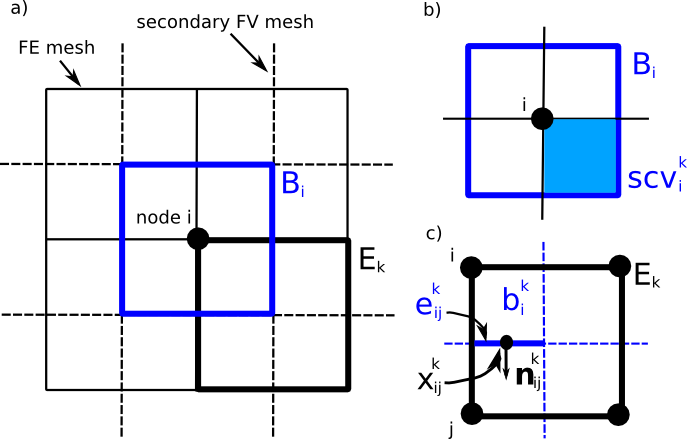
\includegraphics[width=0.8\linewidth,keepaspectratio]{PNG/box_disc.png}
\caption{\label{pc:box} Discretization of the box method}
\end{figure}

The FE mesh divides the box $B_i$ into subcontrolvolumes (scv's) $b^k_i$ (see Figure \ref{pc:box}b). Figure \ref{pc:box}c shows the finite element $E_k$ and the scv's $b^k_i$ inside $E_k$, which belong to four different boxes $B_i$. Also necessary for the discretization are the faces of the subcontrolvolumes (scvf's) $e^k_{ij}$ between the scv's $b^k_i$ and $b^k_j$, where $|e^k_{ij}|$ is the length of the scvf. The integration points $x^k_{ij}$ on $e^k_{ij}$ and the outer normal vector $\mathbf n^k_{ij}$ are also to be defined (see Figure \ref{pc:box}c).

The advantage of the FE method is that unstructured grids can be used, while the FV method is mass conservative. The idea is to apply the FV method (balance of fluxes across the interfaces) to each FV box $B_i$  and to get the fluxes across the interfaces $e^k_{ij}$ at the integration points $x^k_{ij}$ from the FE approach. Consequently, at each scvf the following expression results:

\begin{equation}
 	f(\tilde u(x^k_{ij})) \cdot \mathbf n^k_{ij} \: |e^k_{ij}| \qquad \textrm{with} \qquad \tilde u(x^k_{ij}) = \sum_i N_i(x^k_{ij}) \cdot \hat u_i .
\end{equation}

In the following, the discretization of the balance equation is going to be derived. From the \textsc{Reynolds} transport theorem follows the general balance equation:

\begin{equation}
	\underbrace{\int_G \frac{\partial}{\partial t} \: u \: dG}_{1} + \underbrace{\int_{\partial G} (\mathbf{v} u + \mathbf w) \cdot \textbf n \: d\varGamma}_{2} = \underbrace{\int_G q \: dG}_{3}
\end{equation}

\begin{equation}
	f(u) = \int_G \frac{\partial u}{\partial t} \: dG + \int_{G} \nabla \cdot \underbrace{\left[  \mathbf{v} u + \mathbf w(u)\right] }_{F(u)}  \: dG - \int_G q \: dG = 0
\end{equation}
where term 1 describes the changes of entity $u$ within a control volume over time, term 2 the advective, diffusive and dispersive fluxes over the interfaces of the control volume and term 3 is the source and sink term. $G$ denotes the model domain and $F(u) = F(\mathbf v, p) = F(\mathbf v(x,t), p(x,t))$.

Like the FE method, the box method follows the principle of weighted residuals. In the function $f(u)$ the unknown $u$ is approximated by discrete values at the nodes of the FE mesh $\hat u_i$ and linear basis functions $N_i$ yielding an approximate function $f(\tilde u)$. For $u\in \lbrace \mathbf v, p, x^\kappa \rbrace$ this means

\begin{minipage}[b]{0.47\textwidth}
\begin{equation}
\label{eq:p} 
	\tilde p = \sum_i N_i \hat{p_i}
\end{equation}
\begin{equation}
\label{eq:v} 
	\tilde{\mathbf v} = \sum_i N_i \hat{\mathbf v}
\end{equation}
\begin{equation}
\label{eq:x} 
	\tilde x^\kappa  = \sum_i N_i \hat x^\kappa 
\end{equation}
\end{minipage}
\hfill
\begin{minipage}[b]{0.47\textwidth}
\begin{equation}
\label{eq:dp} 
	\nabla \tilde p = \sum_i \nabla N_i \hat{p_i}
\end{equation}
\begin{equation}
\label{eq:dv} 
	\nabla \tilde{\mathbf v} = \sum_i \nabla N_i \hat{\mathbf v}
\end{equation}
\begin{equation}
\label{eq:dx} 
	\nabla \tilde x^\kappa  = \sum_i \nabla N_i \hat x^\kappa .
\end{equation}
\end{minipage} 

Due to the approximation with node values and basis functions the differential equations are not exactly fulfilled anymore but a residual $\varepsilon$ is produced.

\begin{equation}
	f(u) = 0  \qquad \Rightarrow \qquad f(\tilde u) = \varepsilon
\end{equation}

Application of the principle of weighted residuals, meaning the multiplication of the residual $\varepsilon$ with a weighting function $W_j$  and claiming that this product has to vanish within the whole domain,

\begin{equation}
	\int_G W_j \cdot \varepsilon \: \overset {!}{=} \: 0 \qquad \textrm{with} \qquad \sum_j W_j =1
\end{equation}
yields the following equation:

\begin{equation}
	\int_G W_j \frac{\partial \tilde u}{\partial t} \: dG + \int_G W_j \cdot \left[ \nabla \cdot F(\tilde u) \right]  \: dG - \int_G W_j \cdot q \: dG = \int_G W_j \cdot \varepsilon \: dG \: \overset {!}{=} \: 0 .
\end{equation}

Then, the chain rule and the \textsc{Green-Gaussian} integral theorem are applied.

\begin{equation}
	\int_G W_j \frac{\partial \sum_i N_i \hat u_i}{\partial t} \: dG + \int_{\partial G}  \left[ W_j \cdot F(\tilde u)\right]  \cdot \mathbf n \: d\varGamma_G + \int_G  \nabla W_j \cdot F(\tilde u)  \: dG - \int_G W_j \cdot q \: dG = 0
\end{equation}

A mass lumping technique is applied by assuming that the storage capacity is reduced to the nodes. This means that the integrals $M_{i,j} = \int_G W_j \: N_i \: dG$ are replaced by the mass lumping term $M^{lump}_{i,j}$ which is defined as:

\begin{equation}
	 M^{lump}_{i,j} =\begin{cases} \int_G W_j \: dG = \int_G N_i \: dG = V_i &i = j\\
	0 &i \neq j\\
	         \end{cases}
\end{equation}
where $V_i$ is the volume of the FV box $B_i$ associated with node i. The application of this assumption in combination with $\int_G W_j \:q \: dG = V_i \: q$ yields

\begin{equation}
	V_i \frac{\partial \hat u_i}{\partial t} + \int_{\partial G}  \left[ W_j \cdot F(\tilde u)\right]  \cdot \mathbf n \: d\varGamma_G + \int_G  \nabla W_j \cdot F(\tilde u)  \: dG- V_i \cdot q = 0 \, .
\end{equation}

Defining the weighting function $W_j$ to be piecewisely constant over a control volume box $B_i$ 

\begin{equation}
	W_j(x) = \begin{cases}
	          1 &x \in B_i \\
		  0 &x \notin B_i\\
	         \end{cases}
\end{equation}

causes $\nabla W_j = 0$:

\begin{equation}
\label{eq:disc1} 
	V_i \frac{\partial \hat u_i}{\partial t} + \int_{\partial B_i}  \left[ W_j \cdot F(\tilde u)\right] \cdot \mathbf n  \;  d{\varGamma}_{B_i} - V_i \cdot q = 0 .
\end{equation}

The consideration of the time discretization and inserting $W_j = 1$ finally lead to the discretized form which will be applied to the mathematical flow and transport equations:

\begin{equation}
\label{eq:discfin} 
	V_i \frac{\hat u_i^{n+1} - \hat u_i^{n}}{\Delta t} + \int_{\partial B_i}  F(\tilde u^{n+1}) \cdot \mathbf n  \;  d{\varGamma}_{B_i} - V_i \: q^{n+1} \: = 0 
\end{equation}

\subsection{Cell centered finite volume method - A short introduction}\label{cc}

\begin{figure} [h]
\centering
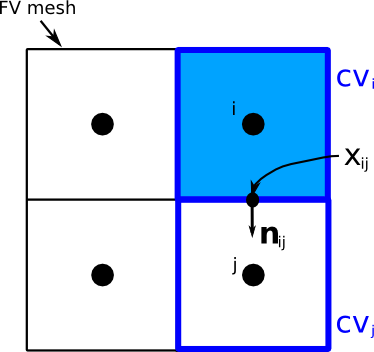
\includegraphics[width=0.4\linewidth,keepaspectratio]{PNG/cc_disc.png}
\caption{\label{pc:cc} Discretization of the cell centered finite volume method}
\end{figure}

The cell centered finite volume method uses the elements of the grid as control volumes. 
For each control volume all discrete values are determined at the element/control volume center (see Figure~\ref{pc:cc}). 
The mass or energy fluxes are evaluated at the integration points ($x_{ij}$), which are located at the midpoints of the control 
volume faces. This is a two point flux approximation since the flux between the element/control volume centers $i$ and $j$ is calculated
only with information from these two points. In contrast the box method uses a multi-point flux approximation where all nodes of the 
element influence the flux between two specific nodes. \\
Neumann boundary conditions are applied at the boundary control volume faces and Dirichlet boundary conditions at the boundary control volumes. \\
The cell centered finite volume method is robust and mass conservative but should only be applied for structured grids 
(the control volume face normal vector ($n_{ij}$) should be parallel to the direction of the gradient between the two element/control 
volume centers). 




\section{Available models} 
The following description of the available models is automatically extracted 
from the Doxygen documentation.
% \textbf{TODO}: Unify notation. 

\subsection{Fully-implicit models}

The fully-implicit models described in this section are using the box or the cell centered finite volume method as described in section \ref{box} and \ref{cc} for spatial and the implicit Euler
method as temporal discretization. The models themselves are located in
subdirectories of \texttt{dumux/implicit} of the \Dumux distribution.

\subsubsection{The single-phase model: OnePModel} 
%%%%%%%%%%%%%%%%%%%%%%%%%%%%%%%%%%%%%%%%%%%%%%%%%%%%%%%%%%%%%%%%%
% This file has been autogenerated from the LaTeX part of the   %
% doxygen documentation; DO NOT EDIT IT! Change the model's .hh %
% file instead!!                                                %
%%%%%%%%%%%%%%%%%%%%%%%%%%%%%%%%%%%%%%%%%%%%%%%%%%%%%%%%%%%%%%%%%

Single-\/phase, isothermal flow model, which uses a standard Darcy approach as the equation for the conservation of momentum\-: \[ v = - \frac{\textbf K}{\mu} \left(\textbf{grad}\, p - \varrho {\textbf g} \right) \]

and solves the mass continuity equation\-: \[ \phi \frac{\partial \varrho}{\partial t} + \text{div} \left\lbrace - \varrho \frac{\textbf K}{\mu} \left( \textbf{grad}\, p -\varrho {\textbf g} \right) \right\rbrace = q, \] All equations are discretized using a vertex-\/centered finite volume (box) or cell-\/centered finite volume scheme as spatial and the implicit Euler method as time discretization. The model supports compressible as well as incompressible fluids.



\subsubsection{The single-phase, two-component model:  OnePTwoCModel} 
%%%%%%%%%%%%%%%%%%%%%%%%%%%%%%%%%%%%%%%%%%%%%%%%%%%%%%%%%%%%%%%%%
% This file has been autogenerated from the LaTeX part of the   %
% doxygen documentation; DO NOT EDIT IT! Change the model's .hh %
% file instead!!                                                %
%%%%%%%%%%%%%%%%%%%%%%%%%%%%%%%%%%%%%%%%%%%%%%%%%%%%%%%%%%%%%%%%%

This model implements a one-\/phase flow of a compressible fluid, that consists of two components, using a standard Darcy approach as the equation for the conservation of momentum\-: \[ v = - \frac{\textbf K}{\mu} \left(\textbf{grad}\, p - \varrho {\textbf g} \right) \]

Gravity can be enabled or disabled via the property system. By inserting this into the continuity equation, one gets \[ \phi\frac{\partial \varrho}{\partial t} - \text{div} \left\{ \varrho \frac{\textbf K}{\mu} \left(\textbf{grad}\, p - \varrho {\textbf g} \right) \right\} = q \;, \]

The transport of the components $\kappa \in \{ w, a \}$ is described by the following equation\-: \[ \phi \frac{ \partial \varrho X^\kappa}{\partial t} - \text{div} \left\lbrace \varrho X^\kappa \frac{{\textbf K}}{\mu} \left( \textbf{grad}\, p - \varrho {\textbf g} \right) + \varrho D^\kappa_\text{pm} \frac{M^\kappa}{M_\alpha} \textbf{grad} x^\kappa \right\rbrace = q. \]

All equations are discretized using a vertex-\/centered finite volume (box) or cell-\/centered finite volume scheme as spatial and the implicit Euler method as time discretization. The model is able to use either mole or mass fractions. The property use\-Moles can be set to either true or false in the problem file. Make sure that the according units are used in the problem setup. use\-Moles is set to true by default.

The primary variables are the pressure $p$ and the mole or mass fraction of dissolved component $x$.



\subsubsection{The two-phase model using the Richards assumption: RichardsModel} 
%%%%%%%%%%%%%%%%%%%%%%%%%%%%%%%%%%%%%%%%%%%%%%%%%%%%%%%%%%%%%%%%%
% This file has been autogenerated from the LaTeX part of the   %
% doxygen documentation; DO NOT EDIT IT! Change the model's .hh %
% file instead!!                                                %
%%%%%%%%%%%%%%%%%%%%%%%%%%%%%%%%%%%%%%%%%%%%%%%%%%%%%%%%%%%%%%%%%

In the unsaturated zone, Richards\textquotesingle{} equation \[ \frac{\partial\;\phi S_w \varrho_w}{\partial t} - \text{div} \left\lbrace \varrho_w \frac{k_{rw}}{\mu_w} \; \mathbf{K} \; \left( \text{\textbf{grad}} p_w - \varrho_w \textbf{g} \right) \right\rbrace = q_w, \] is frequently used to approximate the water distribution above the groundwater level.

It can be derived from the two-\/phase equations, i.\-e. \[ \phi\frac{\partial S_\alpha \varrho_\alpha}{\partial t} - \text{div} \left\lbrace \varrho_\alpha \frac{k_{r\alpha}}{\mu_\alpha}\; \mathbf{K} \; \left( \text{\textbf{grad}} p_\alpha - \varrho_\alpha \textbf{g} \right) \right\rbrace = q_\alpha, \] where $\alpha \in \{w, n\}$ is the fluid phase, $\kappa \in \{ w, a \}$ are the components, $\rho_\alpha$ is the fluid density, $S_\alpha$ is the fluid saturation, $\phi$ is the porosity of the soil, $k_{r\alpha}$ is the relative permeability for the fluid, $\mu_\alpha$ is the fluid\textquotesingle{}s dynamic viscosity, $\mathbf{K}$ is the intrinsic permeability, $p_\alpha$ is the fluid pressure and $g$ is the potential of the gravity field.

In contrast to the full two-\/phase model, the Richards model assumes gas as the non-\/wetting fluid and that it exhibits a much lower viscosity than the (liquid) wetting phase. (For example at atmospheric pressure and at room temperature, the viscosity of air is only about $1\%$ of the viscosity of liquid water.) As a consequence, the $\frac{k_{r\alpha}}{\mu_\alpha}$ term typically is much larger for the gas phase than for the wetting phase. For this reason, the Richards model assumes that $\frac{k_{rn}}{\mu_n}$ is infinitly large. This implies that the pressure of the gas phase is equivalent to the static pressure distribution and that therefore, mass conservation only needs to be considered for the wetting phase.

The model thus choses the absolute pressure of the wetting phase $p_w$ as its only primary variable. The wetting phase saturation is calculated using the inverse of the capillary pressure, i.\-e. \[ S_w = p_c^{-1}(p_n - p_w) \] holds, where $p_n$ is a given reference pressure. Nota bene, that the last step is assumes that the capillary pressure-\/saturation curve can be uniquely inverted, so it is not possible to set the capillary pressure to zero when using the Richards model!



\subsubsection{The two-phase model: TwoPModel}
%%%%%%%%%%%%%%%%%%%%%%%%%%%%%%%%%%%%%%%%%%%%%%%%%%%%%%%%%%%%%%%%%
% This file has been autogenerated from the LaTeX part of the   %
% doxygen documentation; DO NOT EDIT IT! Change the model's .hh %
% file instead!!                                                %
%%%%%%%%%%%%%%%%%%%%%%%%%%%%%%%%%%%%%%%%%%%%%%%%%%%%%%%%%%%%%%%%%

This model implements two-\/phase flow of two immiscible fluids $\alpha \in \{ w, n \}$ using a standard multiphase Darcy approach as the equation for the conservation of momentum, i.\-e. \[ v_\alpha = - \frac{k_{r\alpha}}{\mu_\alpha} \textbf{K} \left(\textbf{grad}\, p_\alpha - \varrho_{\alpha} {\textbf g} \right) \]

By inserting this into the equation for the conservation of the phase mass, one gets \[ \phi \frac{\partial \varrho_\alpha S_\alpha}{\partial t} - \text{div} \left\{ \varrho_\alpha \frac{k_{r\alpha}}{\mu_\alpha} \mathbf{K} \left(\textbf{grad}\, p_\alpha - \varrho_{\alpha} \mbox{\bf g} \right) \right\} - q_\alpha = 0 \;, \]

All equations are discretized using a vertex-\/centered finite volume (box) or cell-\/centered finite volume scheme as spatial and the implicit Euler method as time discretization.

By using constitutive relations for the capillary pressure $p_c = p_n - p_w$ and relative permeability $k_{r\alpha}$ and taking advantage of the fact that $S_w + S_n = 1$, the number of unknowns can be reduced to two. Currently the model supports choosing either $p_w$ and $S_n$ or $p_n$ and $S_w$ as primary variables. The formulation which ought to be used can be specified by setting the {\ttfamily Formulation} property to either {\ttfamily Two\-P\-Common\-Indices\-::p\-Ws\-N} or {\ttfamily Two\-P\-Common\-Indices\-::p\-Ns\-W}. By default, the model uses $p_w$ and $S_n$.



\subsubsection{The two-phase, two-component model: TwoPTwoCModel} 
%%%%%%%%%%%%%%%%%%%%%%%%%%%%%%%%%%%%%%%%%%%%%%%%%%%%%%%%%%%%%%%%%
% This file has been autogenerated from the LaTeX part of the   %
% doxygen documentation; DO NOT EDIT IT! Change the model's .hh %
% file instead!!                                                %
%%%%%%%%%%%%%%%%%%%%%%%%%%%%%%%%%%%%%%%%%%%%%%%%%%%%%%%%%%%%%%%%%

This model implements two-\/phase two-\/component flow of two compressible and partially miscible fluids $\alpha \in \{ w, n \}$ composed of the two components $\kappa \in \{ w, a \}$. The standard multiphase Darcy approach is used as the equation for the conservation of momentum\-: \[ v_\alpha = - \frac{k_{r\alpha}}{\mu_\alpha} \mathbf{K} \left(\textbf{grad}\, p_\alpha - \varrho_{\alpha} \mbox{\bf g} \right) \]

By inserting this into the equations for the conservation of the components, one gets one transport equation for each component \begin{eqnarray*} && \phi \frac{\partial (\sum_\alpha \varrho_\alpha \frac{M^\kappa}{M_\alpha} x_\alpha^\kappa S_\alpha )} {\partial t} - \sum_\alpha \text{div} \left\{ \varrho_\alpha \frac{M^\kappa}{M_\alpha} x_\alpha^\kappa \frac{k_{r\alpha}}{\mu_\alpha} \mathbf{K} (\textbf{grad}\, p_\alpha - \varrho_{\alpha} \mbox{\bf g}) \right\} \nonumber \\ \nonumber \\ &-& \sum_\alpha \text{div} \left\{ D_{\alpha,\text{pm}}^\kappa \varrho_{\alpha} \frac{M^\kappa}{M_\alpha} \textbf{grad} x^\kappa_{\alpha} \right\} - \sum_\alpha q_\alpha^\kappa = 0 \qquad \kappa \in \{w, a\} \, , \alpha \in \{w, g\} \end{eqnarray*}

All equations are discretized using a vertex-\/centered finite volume (box) or cell-\/centered finite volume scheme as spatial and the implicit Euler method as time discretization.

By using constitutive relations for the capillary pressure $p_c = p_n - p_w$ and relative permeability $k_{r\alpha}$ and taking advantage of the fact that $S_w + S_n = 1$ and $x^\kappa_w + x^\kappa_n = 1$, the number of unknowns can be reduced to two. The used primary variables are, like in the two-\/phase model, either $p_w$ and $S_n$ or $p_n$ and $S_w$. The formulation which ought to be used can be specified by setting the {\ttfamily Formulation} property to either Two\-P\-Two\-C\-Indices\-::p\-Ws\-N or Two\-P\-Two\-C\-Indices\-::p\-Ns\-W. By default, the model uses $p_w$ and $S_n$. Moreover, the second primary variable depends on the phase state, since a primary variable switch is included. The phase state is stored for all nodes of the system. The model is able to use either mole or mass fractions. The property use\-Moles can be set to either true or false in the problem file. Make sure that the according units are used in the problem setup. use\-Moles is set to true by default. Following cases can be distinguished\-:
\begin{itemize}
\item Both phases are present\-: The saturation is used (either $S_n$ or $S_w$, dependent on the chosen {\ttfamily Formulation}), as long as $ 0 < S_\alpha < 1$.
\item Only wetting phase is present\-: The mole fraction of, e.\-g., air in the wetting phase $x^a_w$ is used, as long as the maximum mole fraction is not exceeded $(x^a_w<x^a_{w,max})$
\item Only non-\/wetting phase is present\-: The mole fraction of, e.\-g., water in the non-\/wetting phase, $x^w_n$, is used, as long as the maximum mole fraction is not exceeded $(x^w_n<x^w_{n,max})$
\end{itemize}



\subsubsection{The CO2 model: CO2Model} 
%%%%%%%%%%%%%%%%%%%%%%%%%%%%%%%%%%%%%%%%%%%%%%%%%%%%%%%%%%%%%%%%%
% This file has been autogenerated from the LaTeX part of the   %
% doxygen documentation; DO NOT EDIT IT! Change the model's .hh %
% file instead!!                                                %
%%%%%%%%%%%%%%%%%%%%%%%%%%%%%%%%%%%%%%%%%%%%%%%%%%%%%%%%%%%%%%%%%

See \hyperlink{a00633}{Two\-P\-Two\-C\-Model} for reference to the equations used. The \hyperlink{a00074}{C\-O2} model is derived from the 2p2c model. In the \hyperlink{a00074}{C\-O2} model the phase switch criterion is different from the 2p2c model. The phase switch occurs when the equilibrium concentration of a component in a phase is exceeded, instead of the sum of the components in the virtual phase (the phase which is not present) being greater that unity as done in the 2p2c model. The \hyperlink{a00078}{C\-O2\-Volume\-Variables} do not use a constraint solver for calculating the mole fractions as is the case in the 2p2c model. Instead mole fractions are calculated in the Fluid\-System with a given temperature, pressurem and salinity. The model is able to use either mole or mass fractions. The property use\-Moles can be set to either true or false in the problem file. Make sure that the according units are used in the problem setup. use\-Moles is set to false by default.




\subsubsection{The three-phase model: ThreePModel} 
%%%%%%%%%%%%%%%%%%%%%%%%%%%%%%%%%%%%%%%%%%%%%%%%%%%%%%%%%%%%%%%%%
% This file has been autogenerated from the LaTeX part of the   %
% doxygen documentation; DO NOT EDIT IT! Change the model's .hh %
% file instead!!                                                %
%%%%%%%%%%%%%%%%%%%%%%%%%%%%%%%%%%%%%%%%%%%%%%%%%%%%%%%%%%%%%%%%%

This model implements three-\/phase flow of three fluid phases $\alpha \in \{ water, gas, NAPL \}$ The standard multiphase Darcy approach is used as the equation for the conservation of momentum.

By inserting this into the equations for the conservation of the components, the well-\/known multiphase flow equation is obtained.

All equations are discretized using a vertex-\/centered finite volume (box) or cell-\/centered finite volume scheme as spatial and the implicit Euler method as time discretization.

The model uses commonly applied auxiliary conditions like $S_w + S_n + S_g = 1$ for the saturations. Furthermore, the phase pressures are related to each other via capillary pressures between the fluid phases, which are functions of the saturation, e.\-g. according to the approach of Parker et al.

The used primary variables are gas phase pressure $p_g$, water saturation $S_w$ and N\-A\-P\-L saturation $S_n$.



\subsubsection{The three-phase, three-component model: ThreePThreeCModel}
%%%%%%%%%%%%%%%%%%%%%%%%%%%%%%%%%%%%%%%%%%%%%%%%%%%%%%%%%%%%%%%%%
% This file has been autogenerated from the LaTeX part of the   %
% doxygen documentation; DO NOT EDIT IT! Change the model's .hh %
% file instead!!                                                %
%%%%%%%%%%%%%%%%%%%%%%%%%%%%%%%%%%%%%%%%%%%%%%%%%%%%%%%%%%%%%%%%%

This model implements three-\/phase three-\/component flow of three fluid phases $\alpha \in \{ water, gas, NAPL \}$ each composed of up to three components $\kappa \in \{ water, air, contaminant \}$. The standard multiphase Darcy approach is used as the equation for the conservation of momentum\-: \[ v_\alpha = - \frac{k_{r\alpha}}{\mu_\alpha} \mathbf{K} \left(\textbf{grad}\, p_\alpha - \varrho_{\alpha} \mbox{\bf g} \right) \]

By inserting this into the equations for the conservation of the components, one transport equation for each component is obtained as \begin{eqnarray*} && \phi \frac{\partial (\sum_\alpha \varrho_\alpha X_\alpha^\kappa S_\alpha )}{\partial t} - \sum\limits_\alpha \text{div} \left\{ \frac{k_{r\alpha}}{\mu_\alpha} \varrho_\alpha x_\alpha^\kappa \mathbf{K} (\textbf{grad}\, p_\alpha - \varrho_\alpha \mbox{\bf g}) \right\} \nonumber \\ \nonumber \\ && - \sum\limits_\alpha \text{div} \left\{ D_\text{pm}^\kappa \varrho_\alpha \frac{M^\kappa}{M_\alpha} \textbf{grad} x^\kappa_{\alpha} \right\} - q^\kappa = 0 \qquad \forall \kappa , \; \forall \alpha \end{eqnarray*}

Note that these balance equations are molar.

All equations are discretized using a vertex-\/centered finite volume (box) or cell-\/centered finite volume scheme as spatial and the implicit Euler method as time discretization.

The model uses commonly applied auxiliary conditions like $S_w + S_n + S_g = 1$ for the saturations and $x^w_\alpha + x^a_\alpha + x^c_\alpha = 1$ for the mole fractions. Furthermore, the phase pressures are related to each other via capillary pressures between the fluid phases, which are functions of the saturation, e.\-g. according to the approach of Parker et al.

The used primary variables are dependent on the locally present fluid phases. An adaptive primary variable switch is included. The phase state is stored for all nodes of the system. The following cases can be distinguished\-:
\begin{itemize}
\item All three phases are present\-: Primary variables are two saturations $(S_w$ and $S_n)$, and a pressure, in this case $p_g$.
\item Only the water phase is present\-: Primary variables are now the mole fractions of air and contaminant in the water phase $(x_w^a$ and $x_w^c)$, as well as the gas pressure, which is, of course, in a case where only the water phase is present, just the same as the water pressure.
\item Gas and N\-A\-P\-L phases are present\-: Primary variables $(S_n$, $x_g^w$, $p_g)$.
\item Water and N\-A\-P\-L phases are present\-: Primary variables $(S_n$, $x_w^a$, $p_g)$.
\item Only gas phase is present\-: Primary variables $(x_g^w$, $x_g^c$, $p_g)$.
\item Water and gas phases are present\-: Primary variables $(S_w$, $x_w^g$, $p_g)$.
\end{itemize}



\subsubsection{The non-isothermal model: NIModel} 
%%%%%%%%%%%%%%%%%%%%%%%%%%%%%%%%%%%%%%%%%%%%%%%%%%%%%%%%%%%%%%%%%
% This file has been autogenerated from the LaTeX part of the   %
% doxygen documentation; DO NOT EDIT IT! Change the model's .hh %
% file instead!!                                                %
%%%%%%%%%%%%%%%%%%%%%%%%%%%%%%%%%%%%%%%%%%%%%%%%%%%%%%%%%%%%%%%%%

This model implements a generic energy balance for single and multi-\/phase transport problems. Currently the non-\/isothermal model can be used on top of the 1p2c, 2p, 2p2c and 3p3c models. Comparison to simple analytical solutions for pure convective and conductive problems are found in the 1p2c test. Also refer to this test for details on how to activate the non-\/isothermal model.

For the energy balance, local thermal equilibrium is assumed. This results in one energy conservation equation for the porous solid matrix and the fluids\-: \begin{align*} \phi \frac{\partial \sum_\alpha \varrho_\alpha u_\alpha S_\alpha}{\partial t} & + \left( 1 - \phi \right) \frac{\partial (\varrho_s c_s T)}{\partial t} - \sum_\alpha \text{div} \left\{ \varrho_\alpha h_\alpha \frac{k_{r\alpha}}{\mu_\alpha} \mathbf{K} \left( \textbf{grad}\,p_\alpha - \varrho_\alpha \mbox{\bf g} \right) \right\} \\ & - \text{div} \left(\lambda_{pm} \textbf{grad} \, T \right) - q^h = 0. \end{align*} where $h_\alpha$ is the specific enthalpy of a fluid phase $\alpha$ and $u_\alpha = h_\alpha - p_\alpha/\varrho_\alpha$ is the specific internal energy of the phase.



\subsubsection{The $M$-phase, $N$-component model: MpNcModel} 
%%%%%%%%%%%%%%%%%%%%%%%%%%%%%%%%%%%%%%%%%%%%%%%%%%%%%%%%%%%%%%%%%
% This file has been autogenerated from the LaTeX part of the   %
% doxygen documentation; DO NOT EDIT IT! Change the model's .hh %
% file instead!!                                                %
%%%%%%%%%%%%%%%%%%%%%%%%%%%%%%%%%%%%%%%%%%%%%%%%%%%%%%%%%%%%%%%%%

This model implements a $M$-\/phase flow of a fluid mixture composed of $N$ chemical species. The phases are denoted by lower index $\alpha \in \{ 1, \dots, M \}$. All fluid phases are mixtures of $N \geq M - 1$ chemical species which are denoted by the upper index $\kappa \in \{ 1, \dots, N \} $.

The momentum approximation can be selected via \char`\"{}\-Base\-Flux\-Variables\char`\"{}\-: Darcy (\hyperlink{a00278}{Implicit\-Darcy\-Flux\-Variables}) and Forchheimer (\hyperlink{a00279}{Implicit\-Forchheimer\-Flux\-Variables}) relations are available for all Box models.

By inserting this into the equations for the conservation of the mass of each component, one gets one mass-\/continuity equation for each component $\kappa$ \[ \sum_{\kappa} \left( \phi \frac{\partial \left(\varrho_\alpha x_\alpha^\kappa S_\alpha\right)}{\partial t} + \mathrm{div}\; \left\{ v_\alpha \frac{\varrho_\alpha}{\overline M_\alpha} x_\alpha^\kappa \right\} \right) = q^\kappa \] with $\overline M_\alpha$ being the average molar mass of the phase $\alpha$\-: \[ \overline M_\alpha = \sum_\kappa M^\kappa \; x_\alpha^\kappa \]

For the missing $M$ model assumptions, the model assumes that if a fluid phase is not present, the sum of the mole fractions of this fluid phase is smaller than $1$, i.\-e. \[ \forall \alpha: S_\alpha = 0 \implies \sum_\kappa x_\alpha^\kappa \leq 1 \]

Also, if a fluid phase may be present at a given spatial location its saturation must be positive\-: \[ \forall \alpha: \sum_\kappa x_\alpha^\kappa = 1 \implies S_\alpha \geq 0 \]

Since at any given spatial location, a phase is always either present or not present, one of the strict equalities on the right hand side is always true, i.\-e. \[ \forall \alpha: S_\alpha \left( \sum_\kappa x_\alpha^\kappa - 1 \right) = 0 \] always holds.

These three equations constitute a non-\/linear complementarity problem, which can be solved using so-\/called non-\/linear complementarity functions $\Phi(a, b)$ which have the property \[\Phi(a,b) = 0 \iff a \geq0 \land b \geq0 \land a \cdot b = 0 \]

Several non-\/linear complementarity functions have been suggested, e.\-g. the Fischer-\/\-Burmeister function \[ \Phi(a,b) = a + b - \sqrt{a^2 + b^2} \;. \] This model uses \[ \Phi(a,b) = \min \{a, b \}\;, \] because of its piecewise linearity.

These equations are then discretized using a fully-\/implicit vertex centered finite volume scheme (often known as 'box'-\/scheme) for spatial discretization and the implicit Euler method as temporal discretization.

The model assumes local thermodynamic equilibrium and uses the following primary variables\-:
\begin{itemize}
\item The component fugacities $f^1, \dots, f^{N}$
\item The pressure of the first phase $p_1$
\item The saturations of the first $M-1$ phases $S_1, \dots, S_{M-1}$
\item Temperature $T$ if the energy equation is enabled
\end{itemize}



\subsubsection{The two-phase, discrete fracture model: TwoPDFMModel} 
%%%%%%%%%%%%%%%%%%%%%%%%%%%%%%%%%%%%%%%%%%%%%%%%%%%%%%%%%%%%%%%%%
% This file has been autogenerated from the LaTeX part of the   %
% doxygen documentation; DO NOT EDIT IT! Change the model's .hh %
% file instead!!                                                %
%%%%%%%%%%%%%%%%%%%%%%%%%%%%%%%%%%%%%%%%%%%%%%%%%%%%%%%%%%%%%%%%%

This model implements two-\/phase flow of two immiscible fluids $\alpha \in \{ w, n \}$ using a standard multiphase Darcy approach as the equation for the conservation of momentum, i.\-e. \[ v_\alpha = - \frac{k_{r\alpha}}{\mu_\alpha} \textbf{K} \left(\textbf{grad}\, p_\alpha - \varrho_{\alpha} {\textbf g} \right) \]

By inserting this into the equation for the conservation of the phase mass, one gets \[ \phi \frac{\partial \varrho_\alpha S_\alpha}{\partial t} - \text{div} \left\{ \varrho_\alpha \frac{k_{r\alpha}}{\mu_\alpha} \mathbf{K} \left(\textbf{grad}\, p_\alpha - \varrho_{\alpha} \mbox{\bf g} \right) \right\} - q_\alpha = 0 \;, \]

These equations are discretized by a fully-\/coupled vertex centered finite volume (box) scheme as spatial and the implicit Euler method as time discretization.

By using constitutive relations for the capillary pressure $p_c = p_n - p_w$ and relative permeability $k_{r\alpha}$ and taking advantage of the fact that $S_w + S_n = 1$, the number of unknowns can be reduced to two. Currently the model supports choosing either $p_w$ and $S_n$ or $p_n$ and $S_w$ as primary variables. The formulation which ought to be used can be specified by setting the {\ttfamily Formulation} property to either {\ttfamily Two\-P\-Common\-Indices\-::p\-Ws\-N} or {\ttfamily Two\-P\-Common\-Indices\-::p\-Ns\-W}. By default, the model uses $p_w$ and $S_n$.



\subsubsection{The Stokes model: StokesModel} 
%%%%%%%%%%%%%%%%%%%%%%%%%%%%%%%%%%%%%%%%%%%%%%%%%%%%%%%%%%%%%%%%%
% This file has been autogenerated from the LaTeX part of the   %
% doxygen documentation; DO NOT EDIT IT! Change the model's .hh %
% file instead!!                                                %
%%%%%%%%%%%%%%%%%%%%%%%%%%%%%%%%%%%%%%%%%%%%%%%%%%%%%%%%%%%%%%%%%

This model implements laminar Stokes flow of a single fluid, solving the momentum balance equation \[ \frac{\partial \left(\varrho_g {\boldsymbol{v}}_g\right)}{\partial t} + \boldsymbol{\nabla} \boldsymbol{\cdot} \left(p_g {\bf {I}} - \mu_g \left(\boldsymbol{\nabla} \boldsymbol{v}_g + \boldsymbol{\nabla} \boldsymbol{v}_g^T\right)\right) - \varrho_g {\bf g} = 0, \]

and the mass balance equation \[ \frac{\partial \varrho_g}{\partial t} + \boldsymbol{\nabla}\boldsymbol{\cdot}\left(\varrho_g {\boldsymbol{v}}_g\right) - q_g = 0. \]

By setting the property {\ttfamily Enable\-Navier\-Stokes} to {\ttfamily true} the Navier-\/\-Stokes equation can be solved. In this case an additional term \[ \varrho_g \left(\boldsymbol{v}_g \boldsymbol{\cdot} \boldsymbol{\nabla} \right) \boldsymbol{v}_g \] is added to the momentum balance equation.

This is discretized by a fully-\/coupled vertex-\/centered finite volume (box) scheme in space and by the implicit Euler method in time.



\subsubsection{The isothermal $N$-component Stokes model: StokesNcModel} 
%%%%%%%%%%%%%%%%%%%%%%%%%%%%%%%%%%%%%%%%%%%%%%%%%%%%%%%%%%%%%%%%%
% This file has been autogenerated from the LaTeX part of the   %
% doxygen documentation; DO NOT EDIT IT! Change the model's .hh %
% file instead!!                                                %
%%%%%%%%%%%%%%%%%%%%%%%%%%%%%%%%%%%%%%%%%%%%%%%%%%%%%%%%%%%%%%%%%

This model implements an isothermal n-\/component Stokes flow of a fluid solving a momentum balance, a mass balance and a conservation equation for each component. When using mole fractions naturally the densities represent molar densites

Momentum Balance\-: \[ \frac{\partial \left(\varrho_g {\boldsymbol{v}}_g\right)}{\partial t} + \boldsymbol{\nabla} \boldsymbol{\cdot} \left(p_g {\bf {I}} - \mu_g \left(\boldsymbol{\nabla} \boldsymbol{v}_g + \boldsymbol{\nabla} \boldsymbol{v}_g^T\right)\right) - \varrho_g {\bf g} = 0, \]

Mass balance equation\-: \[ \frac{\partial \varrho_g}{\partial t} + \boldsymbol{\nabla}\boldsymbol{\cdot}\left(\varrho_g {\boldsymbol{v}}_g\right) - q_g = 0 \]

\hyperlink{a00084}{Component} mass balance equations\-: \[ \frac{\partial \left(\varrho_g X_g^\kappa\right)}{\partial t} + \boldsymbol{\nabla} \boldsymbol{\cdot} \left( \varrho_g {\boldsymbol{v}}_g X_g^\kappa - D^\kappa_g \varrho_g \boldsymbol{\nabla} X_g^\kappa \right) - q_g^\kappa = 0 \]

This is discretized using a fully-\/coupled vertex centered finite volume (box) scheme as spatial and the implicit Euler method in time.



\subsubsection{The non-isothermal $N$-component Stokes model: StokesNcNIModel} 
%%%%%%%%%%%%%%%%%%%%%%%%%%%%%%%%%%%%%%%%%%%%%%%%%%%%%%%%%%%%%%%%%
% This file has been autogenerated from the LaTeX part of the   %
% doxygen documentation; DO NOT EDIT IT! Change the model's .hh %
% file instead!!                                                %
%%%%%%%%%%%%%%%%%%%%%%%%%%%%%%%%%%%%%%%%%%%%%%%%%%%%%%%%%%%%%%%%%

This model implements a non-\/isothermal n-\/component Stokes flow of a fluid solving a momentum balance, a mass balance, a conservation equation for one component, and one balance equation for the energy.

Momentum Balance\-: \[ \frac{\partial \left(\varrho_g {\boldsymbol{v}}_g\right)}{\partial t} + \boldsymbol{\nabla} \boldsymbol{\cdot} \left(p_g {\bf {I}} - \mu_g \left(\boldsymbol{\nabla} \boldsymbol{v}_g + \boldsymbol{\nabla} \boldsymbol{v}_g^T\right)\right) - \varrho_g {\bf g} = 0, \]

Mass balance equation\-: \[ \frac{\partial \varrho_g}{\partial t} + \boldsymbol{\nabla}\boldsymbol{\cdot}\left(\varrho_g {\boldsymbol{v}}_g\right) - q_g = 0 \]

\hyperlink{a00088}{Component} mass balance equation\-: \[ \frac{\partial \left(\varrho_g X_g^\kappa\right)}{\partial t} + \boldsymbol{\nabla} \boldsymbol{\cdot} \left( \varrho_g {\boldsymbol{v}}_g X_g^\kappa - D^\kappa_g \varrho_g \frac{M^\kappa}{M_g} \boldsymbol{\nabla} x_g^\kappa \right) - q_g^\kappa = 0 \]

Energy balance equation\-: \[ \frac{\partial (\varrho_g u_g)}{\partial t} + \boldsymbol{\nabla} \boldsymbol{\cdot} \left( \varrho_g h_g {\boldsymbol{v}}_g - \sum_\kappa \left[ h^\kappa_g D^\kappa_g \varrho_g \frac{M^\kappa}{M_g} \nabla x^\kappa_g \right] - \lambda_g \boldsymbol{\nabla} T \right) - q_T = 0 \]

This is discretized using a fully-\/coupled vertex centered finite volume (box) scheme as spatial and the implicit Euler method as temporal discretization.



\subsubsection{The linear elastic model: ElasticModel} 
%%%%%%%%%%%%%%%%%%%%%%%%%%%%%%%%%%%%%%%%%%%%%%%%%%%%%%%%%%%%%%%%%
% This file has been autogenerated from the LaTeX part of the   %
% doxygen documentation; DO NOT EDIT IT! Change the model's .hh %
% file instead!!                                                %
%%%%%%%%%%%%%%%%%%%%%%%%%%%%%%%%%%%%%%%%%%%%%%%%%%%%%%%%%%%%%%%%%

This model implements a linear elastic solid using Hooke\textquotesingle{}s law as stress-\/strain relation and a quasi-\/stationary momentum balance equation\-: \[ \boldsymbol{\sigma} = 2\,G\,\boldsymbol{\epsilon} + \lambda \,\text{tr} (\boldsymbol{\epsilon}) \, \boldsymbol{I}. \]

with the strain tensor $\boldsymbol{\epsilon}$ as a function of the solid displacement gradient $\textbf{grad} \boldsymbol{u}$\-: \[ \boldsymbol{\epsilon} = \frac{1}{2} \, (\textbf{grad} \boldsymbol{u} + \textbf{grad}^T \boldsymbol{u}). \]

Gravity can be enabled or disabled via the property system. By inserting this into the momentum balance equation, one gets \[ \text{div} \boldsymbol{\sigma} + \varrho {\textbf g} = 0 \;, \]

The equation is discretized using a vertex-\/centered finite volume (box) scheme as spatial discretization.



\subsubsection{The linear elastic one-phase two-component model: ElOnePTwoCModel} 
%%%%%%%%%%%%%%%%%%%%%%%%%%%%%%%%%%%%%%%%%%%%%%%%%%%%%%%%%%%%%%%%%
% This file has been autogenerated from the LaTeX part of the   %
% doxygen documentation; DO NOT EDIT IT! Change the model's .hh %
% file instead!!                                                %
%%%%%%%%%%%%%%%%%%%%%%%%%%%%%%%%%%%%%%%%%%%%%%%%%%%%%%%%%%%%%%%%%

This model implements a one-\/phase flow of an incompressible fluid, that consists of two components. The deformation of the solid matrix is described with a quasi-\/stationary momentum balance equation. The influence of the pore fluid is accounted for through the effective stress concept (Biot 1941). The total stress acting on a rock is partially supported by the rock matrix and partially supported by the pore fluid. The effective stress represents the share of the total stress which is supported by the solid rock matrix and can be determined as a function of the strain according to Hooke\textquotesingle{}s law.

As an equation for the conservation of momentum within the fluid phase Darcy\textquotesingle{}s approach is used\-: \[ v = - \frac{\textbf K}{\mu} \left(\textbf{grad}\, p - \varrho_w {\textbf g} \right) \]

Gravity can be enabled or disabled via the property system. By inserting this into the volume balance of the solid-\/fluid mixture, one gets \[ \frac{\partial \text{div} \textbf{u}}{\partial t} - \text{div} \left\{ \frac{\textbf K}{\mu} \left(\textbf{grad}\, p - \varrho_w {\textbf g} \right)\right\} = q \;, \]

The transport of the components $\kappa \in \{ w, a \}$ is described by the following equation\-: \[ \frac{ \partial \phi_{eff} X^\kappa}{\partial t} - \text{div} \left\lbrace X^\kappa \frac{{\textbf K}}{\mu} \left( \textbf{grad}\, p - \varrho_w {\textbf g} \right) + D^\kappa_\text{pm} \frac{M^\kappa}{M_\alpha} \textbf{grad} x^\kappa - \phi_{eff} X^\kappa \frac{\partial \boldsymbol{u}}{\partial t} \right\rbrace = q. \]

If the model encounters stability problems, a stabilization term can be switched on. The stabilization term is defined in Aguilar et al (2008)\-: \[ \beta \text{div} \textbf{grad} \frac{\partial p}{\partial t} \] with $\beta$\-: \[ \beta = h^2 / 4(\lambda + 2 \mu) \] where $h$ is the discretization length.

The balance equations with the stabilization term are given below\-: \[ \frac{\partial \text{div} \textbf{u}}{\partial t} - \text{div} \left\{ \frac{\textbf K}{\mu} \left(\textbf{grad}\, p - \varrho_w {\textbf g} \right) + \varrho_w \beta \textbf{grad} \frac{\partial p}{\partial t} \right\} = q \;, \]

The transport of the components $\kappa \in \{ w, a \}$ is described by the following equation\-:

\[ \frac{ \partial \phi_{eff} X^\kappa}{\partial t} - \text{div} \left\lbrace X^\kappa \frac{{\textbf K}}{\mu} \left( \textbf{grad}\, p - \varrho_w {\textbf g} \right) + \varrho_w X^\kappa \beta \textbf{grad} \frac{\partial p}{\partial t} + D^\kappa_\text{pm} \frac{M^\kappa}{M_\alpha} \textbf{grad} x^\kappa - \phi_{eff} X^\kappa \frac{\partial \boldsymbol{u}}{\partial t} \right\rbrace = q. \]

The quasi-\/stationary momentum balance equation is\-: \[ \text{div}\left( \boldsymbol{\sigma'}- p \boldsymbol{I} \right) + \left( \phi_{eff} \varrho_w + (1 - \phi_{eff}) * \varrho_s \right) {\textbf g} = 0 \;, \] with the effective stress\-: \[ \boldsymbol{\sigma'} = 2\,G\,\boldsymbol{\epsilon} + \lambda \,\text{tr} (\boldsymbol{\epsilon}) \, \boldsymbol{I}. \]

and the strain tensor $\boldsymbol{\epsilon}$ as a function of the solid displacement gradient $\textbf{grad} \boldsymbol{u}$\-: \[ \boldsymbol{\epsilon} = \frac{1}{2} \, (\textbf{grad} \boldsymbol{u} + \textbf{grad}^T \boldsymbol{u}). \]

Here, the rock mechanics sign convention is switch off which means compressive stresses are $<$ 0 and tensile stresses are $>$ 0. The rock mechanics sign convention can be switched on for the vtk output via the property system.

The effective porosity is calculated as a function of the solid displacement\-: \[ \phi_{eff} = \frac{\phi_{init} + \text{div} \boldsymbol{u}}{1 + \text{div}} \] All equations are discretized using a vertex-\/centered finite volume (box) or cell-\/centered finite volume scheme as spatial and the implicit Euler method as time discretization.

The primary variables are the pressure $p$ and the mole or mass fraction of dissolved component $x$ and the solid displacement vector $\boldsymbol{u}$.



\subsubsection{The linear elastic two-phase model: ElTwoPModel} 
%%%%%%%%%%%%%%%%%%%%%%%%%%%%%%%%%%%%%%%%%%%%%%%%%%%%%%%%%%%%%%%%%
% This file has been autogenerated from the LaTeX part of the   %
% doxygen documentation; DO NOT EDIT IT! Change the model's .hh %
% file instead!!                                                %
%%%%%%%%%%%%%%%%%%%%%%%%%%%%%%%%%%%%%%%%%%%%%%%%%%%%%%%%%%%%%%%%%

This model implements a two-\/phase flow of compressible immiscible fluids $\alpha \in \{ w, n \}$. The deformation of the solid matrix is described with a quasi-\/stationary momentum balance equation. The influence of the pore fluid is accounted for through the effective stress concept (Biot 1941). The total stress acting on a rock is partially supported by the rock matrix and partially supported by the pore fluid. The effective stress represents the share of the total stress which is supported by the solid rock matrix and can be determined as a function of the strain according to Hooke\textquotesingle{}s law.

As an equation for the conservation of momentum within the fluid phases the standard multiphase Darcy\textquotesingle{}s approach is used\-: \[ v_\alpha = - \frac{k_{r\alpha}}{\mu_\alpha} \textbf{K} \left(\textbf{grad}\, p_\alpha - \varrho_{\alpha} {\textbf g} \right) \]

Gravity can be enabled or disabled via the property system. By inserting this into the continuity equation, one gets \[ \frac{\partial \phi_{eff} \varrho_\alpha S_\alpha}{\partial t} - \text{div} \left\{ \varrho_\alpha \frac{k_{r\alpha}}{\mu_\alpha} \mathbf{K}_\text{eff} \left(\textbf{grad}\, p_\alpha - \varrho_{\alpha} \mathbf{g} \right) - \phi_{eff} \varrho_\alpha S_\alpha \frac{\partial \mathbf{u}}{\partial t} \right\} - q_\alpha = 0 \;, \]

A quasi-\/stationary momentum balance equation is solved for the changes with respect to the initial conditions (Darcis 2012), note that this implementation assumes the soil mechanics sign convention (i.\-e. compressive stresses are negative)\-: \[ \text{div}\left( \boldsymbol{\Delta \sigma'}- \Delta p_{eff} \boldsymbol{I} \right) + \Delta \varrho_b {\textbf g} = 0 \;, \] with the effective stress\-: \[ \boldsymbol{\sigma'} = 2\,G\,\boldsymbol{\epsilon} + \lambda \,\text{tr} (\boldsymbol{\epsilon}) \, \mathbf{I}. \]

and the strain tensor $\boldsymbol{\epsilon}$ as a function of the solid displacement gradient $\textbf{grad} \mathbf{u}$\-: \[ \boldsymbol{\epsilon} = \frac{1}{2} \, (\textbf{grad} \mathbf{u} + \textbf{grad}^T \mathbf{u}). \]

Here, the rock mechanics sign convention is switch off which means compressive stresses are $<$ 0 and tensile stresses are $>$ 0. The rock mechanics sign convention can be switched on for the vtk output via the property system.

The effective porosity and the effective permeability are calculated as a function of the solid displacement\-: \[ \phi_{eff} = \frac{\phi_{init} + \text{div} \mathbf{u}}{1 + \text{div} \mathbf{u}} \] \[ K_{eff} = K_{init} \text{exp}\left( 22.2(\phi_{eff}/\phi_{init} -1 )\right) \] The mass balance equations are discretized using a vertex-\/centered finite volume (box) or cell-\/centered finite volume scheme as spatial and the implicit Euler method as time discretization. The momentum balance equations are discretized using a standard Galerkin Finite Element method as spatial discretization scheme.

The primary variables are the wetting phase pressure $p_w$, the nonwetting phase saturation $S_n$ and the solid displacement vector $\mathbf{u}$ (changes in solid displacement with respect to initial conditions).



\subsection{Decoupled models}
%
The basic idea the so-called decoupled models have in common is to reformulate the equations of multi-phase flow (e.g. Eq. \ref{A3:eqmass1}) into one equation for pressure and equations for phase-/component-/etc. transport. The pressure equation is the sum of the mass balance equations and thus considers the total flow of the fluid system. The new set of equations is considered as decoupled (or weakly coupled) and can thus be solved sequentially. The most popular decoupled model is the so-called fractional flow formulation for two-phase flow which is usually implemented applying an IMplicit Pressure Explicit Saturation algorithm (IMPES).
In comparison to a fully implicit model, the decoupled structure allows the use of different discretization methods for the different equations. The standard method used in the decoupled models is a cell centered finite volume method. Further schemes, so far only available for the two-phase pressure equation, are cell centered finite volumes with multi-point flux approximation (MPFA O-method) and mimetic finite differences.

An $h$-adaptive implementation of both \nameref{ch:2p_decoupled} and \nameref{ch:2p2c_decoupled} is provided for two dimensions.
%
\subsubsection{The one-phase model}
%%%%%%%%%%%%%%%%%%%%%%%%%%%%%%%%%%%%%%%%%%%%%%%%%%%%%%%%%%%%%%%%%
% This file has been autogenerated from the LaTeX part of the   %
% doxygen documentation; DO NOT EDIT IT! Change the model's .hh %
% file instead!!                                                %
%%%%%%%%%%%%%%%%%%%%%%%%%%%%%%%%%%%%%%%%%%%%%%%%%%%%%%%%%%%%%%%%%

\-This model solves equations of the form \[ \textbf{div}\, \boldsymbol v = q. \] \-The velocity $ \boldsymbol v $ is the single phase \-Darcy velocity\-: \[ \boldsymbol v = -\frac{1}{\mu} \boldsymbol K \left(\textbf{grad}\, p + \rho \, g \, \textbf{grad}\, z\right), \] where $ p $ is the pressure, $ \boldsymbol K $ the absolute permeability, $ \mu $ the viscosity, $ \rho $ the density, and $ g $ the gravity constant, and $ q $ is the source term. \-At the boundary, $ p = p_D $ on $ \Gamma_{Dirichlet} $, and $ \boldsymbol v \cdot \boldsymbol n = q_N$ on $ \Gamma_{Neumann} $.




\subsubsection{The two-phase model}\label{ch:2p_decoupled}

\paragraph{Pressure model}
%%%%%%%%%%%%%%%%%%%%%%%%%%%%%%%%%%%%%%%%%%%%%%%%%%%%%%%%%%%%%%%%%
% This file has been autogenerated from the LaTeX part of the   %
% doxygen documentation; DO NOT EDIT IT! Change the model's .hh %
% file instead!!                                                %
%%%%%%%%%%%%%%%%%%%%%%%%%%%%%%%%%%%%%%%%%%%%%%%%%%%%%%%%%%%%%%%%%

This model solves equations of the form \[ \phi \left( \rho_w \frac{\partial S_w}{\partial t} + \rho_n \frac{\partial S_n}{\partial t}\right) + \text{div}\, \boldsymbol{v}_{total} = q. \] The definition of the total velocity $\boldsymbol{v}_{total}$ depends on the choice of the primary pressure variable. Further, fluids can be assumed to be compressible or incompressible (Property\-: {\ttfamily Enable\-Compressibility}). In the incompressible case a wetting $(w) $ phase pressure as primary variable leads to

\[ - \text{div}\, \left[\lambda \boldsymbol K \left(\textbf{grad}\, p_w + f_n \textbf{grad}\, p_c + \sum f_\alpha \rho_\alpha \, g \, \textbf{grad}\, z\right)\right] = q, \]

a non-\/wetting ( $ n $) phase pressure yields \[ - \text{div}\, \left[\lambda \boldsymbol K \left(\textbf{grad}\, p_n - f_w \textbf{grad}\, p_c + \sum f_\alpha \rho_\alpha \, g \, \textbf{grad}\, z\right)\right] = q, \] and a global pressure leads to \[ - \text{div}\, \left[\lambda \boldsymbol K \left(\textbf{grad}\, p_{global} + \sum f_\alpha \rho_\alpha \, g \, \textbf{grad}\, z\right)\right] = q. \] Here, $ p_\alpha $ is a phase pressure, $ p_ {global} $ the global pressure of a classical fractional flow formulation (see e.\-g. P. Binning and M. A. Celia, ''Practical implementation of the fractional flow approach to multi-\/phase flow simulation'', Advances in water resources, vol. 22, no. 5, pp. 461-\/478, 1999.), $ p_c = p_n - p_w $ is the capillary pressure, $ \boldsymbol K $ the absolute permeability, $ \lambda = \lambda_w + \lambda_n $ the total mobility depending on the saturation ( $ \lambda_\alpha = k_{r_\alpha} / \mu_\alpha $), $ f_\alpha = \lambda_\alpha / \lambda $ the fractional flow function of a phase, $ \rho_\alpha $ a phase density, $ g $ the gravity constant and $ q $ the source term.

For all cases, $ p = p_D $ on $ \Gamma_{Dirichlet} $, and $ \boldsymbol v_{total} \cdot \boldsymbol n = q_N $ on $ \Gamma_{Neumann} $.

The slightly compressible case is only implemented for phase pressures! In this case for a wetting $(w) $ phase pressure as primary variable the equations are formulated as \[ \phi \left( \rho_w \frac{\partial S_w}{\partial t} + \rho_n \frac{\partial S_n}{\partial t}\right) - \text{div}\, \left[\lambda \boldsymbol{K} \left(\textbf{grad}\, p_w + f_n \, \textbf{grad}\, p_c + \sum f_\alpha \rho_\alpha \, g \, \textbf{grad}\, z\right)\right] = q, \] and for a non-\/wetting ( $ n $) phase pressure as \[ \phi \left( \rho_w \frac{\partial S_w}{\partial t} + \rho_n \frac{\partial S_n}{\partial t}\right) - \text{div}\, \left[\lambda \boldsymbol{K} \left(\textbf{grad}\, p_n - f_w \textbf{grad}\, p_c + \sum f_\alpha \rho_\alpha \, g \, \textbf{grad}\, z\right)\right] = q, \] In this slightly compressible case the following definitions are valid\-: $ \lambda = \rho_w \lambda_w + \rho_n \lambda_n $, $ f_\alpha = (\rho_\alpha \lambda_\alpha) / \lambda $ This model assumes that temporal changes in density are very small and thus terms of temporal derivatives are negligible in the pressure equation. Depending on the formulation the terms including time derivatives of saturations are simplified by inserting $ S_w + S_n = 1 $.

In the I\-M\-P\-E\-S models the default setting is\-:


\begin{itemize}
\item formulation\-: $ p_w-S_w $ (Property\-: {\itshape Formulation} defined as {\itshape \hyperlink{a00095_a601a847774d6e1b2e2a2b469f70c3f22}{Decoupled\-Two\-P\-Common\-Indices\-::pwsw}})
\item compressibility\-: disabled (Property\-: {\itshape Enable\-Compressibility} set to {\itshape false})
\end{itemize}




\paragraph{Saturation model}
%%%%%%%%%%%%%%%%%%%%%%%%%%%%%%%%%%%%%%%%%%%%%%%%%%%%%%%%%%%%%%%%%
% This file has been autogenerated from the LaTeX part of the   %
% doxygen documentation; DO NOT EDIT IT! Change the model's .hh %
% file instead!!                                                %
%%%%%%%%%%%%%%%%%%%%%%%%%%%%%%%%%%%%%%%%%%%%%%%%%%%%%%%%%%%%%%%%%

This model solves equations of the form

\[ \phi \frac{\partial (\rho_\alpha S_\alpha)}{\partial t} + \text{div}\, (\rho_\alpha \boldsymbol{v_\alpha}) = q_\alpha, \]

where $ S_\alpha $ is the saturation of phase $ \alpha $ (wetting $(w) $, non-\/wetting $(n) $) and $ \boldsymbol v_\alpha $ is the phase velocity defined by the multi-\/phase Darcy equation. If a phase velocity is reconstructed from the pressure solution it can be directly inserted into the previous equation. In the incompressible case the equation is further divided by the phase density $ \rho_\alpha $. If a total velocity is reconstructed the saturation equation is reformulated into\-:

\[ \phi \frac{\partial S_w}{\partial t} + f_w \text{div}\, \boldsymbol{v}_{t} + f_w \lambda_n \boldsymbol{K}\left(\textbf{grad}\, p_c + (\rho_n-\rho_w) \, g \, \textbf{grad} z \right)= q_\alpha, \] to get a wetting phase saturation or \[ \phi \frac{\partial S_n}{\partial t} + f_n \text{div}\, \boldsymbol{v}_{t} - f_n \lambda_w \boldsymbol{K}\left(\textbf{grad}\, p_c + (\rho_n-\rho_w) \, g \, \textbf{grad} z \right)= q_\alpha, \] if the non-\/wetting phase saturation is the primary transport variable.

The total velocity formulation is only implemented for incompressible fluids and $ f_\alpha $ is the fractional flow function, $ \lambda_\alpha $ is the mobility, $ \boldsymbol K $ the absolute permeability, $ p_c $ the capillary pressure, $ \rho $ the fluid density, $ g $ the gravity constant, and $ q $ the source term.

In the I\-M\-P\-E\-S models the default setting is\-:

formulation\-: $ p_w $ -\/ $ S_w $ (Property\-: {\itshape Formulation} defined as {\itshape \hyperlink{a00080_a04294fbcf0af5328016a160dbd8bfff9}{Decoupled\-Two\-P\-Common\-Indices\-::pw\-Sw}})

compressibility\-: disabled (Property\-: {\itshape Enable\-Compressibility} set to {\itshape false})




\subsubsection{The two-phase, two-component model}\label{ch:2p2c_decoupled}
%%%%%%%%%%%%%%%%%%%%%%%%%%%%%%%%%%%%%%%%%%%%%%%%%%%%%%%%%%%%%%%%%
% This file has been autogenerated from the LaTeX part of the   %
% doxygen documentation; DO NOT EDIT IT! Change the model's .hh %
% file instead!!                                                %
%%%%%%%%%%%%%%%%%%%%%%%%%%%%%%%%%%%%%%%%%%%%%%%%%%%%%%%%%%%%%%%%%

Provides a Finite Volume implementation for the pressure equation of a compressible system with two components. An I\-M\-P\-E\-S-\/like method is used for the sequential solution of the problem. Diffusion is neglected, capillarity can be regarded. Isothermal conditions and local thermodynamic equilibrium are assumed. Gravity is included. \[ c_{total}\frac{\partial p}{\partial t} + \sum_{\kappa} \frac{\partial v_{total}}{\partial C^{\kappa}} \nabla \cdot \left( \sum_{\alpha} X^{\kappa}_{\alpha} \varrho_{\alpha} \bf{v}_{\alpha}\right) = \sum_{\kappa} \frac{\partial v_{total}}{\partial C^{\kappa}} q^{\kappa}, \] where $\bf{v}_{\alpha} = - \lambda_{\alpha} \bf{K} \left(\nabla p_{\alpha} + \rho_{\alpha} \bf{g} \right) $. $ c_{total} $ represents the total compressibility, for constant porosity this yields $ - \frac{\partial V_{total}}{\partial p_{\alpha}} $, $p_{\alpha} $ denotes the phase pressure, $ \bf{K} $ the absolute permeability, $ \lambda_{\alpha} $ the phase mobility, $ \rho_{\alpha} $ the phase density and $ \bf{g} $ the gravity constant and $ C^{\kappa} $ the total \hyperlink{a00070}{Component} concentration. See paper S\-P\-E 99619 or \char`\"{}\-Analysis of a Compositional Model for Fluid
Flow in Porous Media\char`\"{} by Chen, Qin and Ewing for derivation.

The pressure base class \hyperlink{a00131}{F\-V\-Pressure} assembles the matrix and right-\/hand-\/side vector and solves for the pressure vector, whereas this class provides the actual entries for the matrix and R\-H\-S vector. The partial derivatives of the actual fluid volume $ v_{total} $ are gained by using a secant method.



%%%%%%%%%%%%%%%%%%%%%%%%%%%%%%%%%%%%%%%%%%%%%%%%%%%%%%%%%%%%%%%%%
% This file is NOT autogenerated                                %
%%%%%%%%%%%%%%%%%%%%%%%%%%%%%%%%%%%%%%%%%%%%%%%%%%%%%%%%%%%%%%%%%

The transport step is described by the finite volume model for the solution of the transport equation for compositional two-\/phase flow.
\[ \frac{\partial C^\kappa}{\partial t} = - \nabla \cdot \left( \sum_{\alpha} X^{\kappa}_{\alpha} \varrho_{\alpha} \bf{v}_{\alpha}\right) + q^{\kappa}, \]
where $ \bf{v}_{\alpha} = - \lambda_{\alpha} \bf{K} \left(\nabla p_{\alpha} + \rho_{\alpha} \bf{g} \right) $. $ p_{\alpha} $ denotes the phase pressure, 
$ \bf{K} $ the absolute permeability, 
$ \lambda_{\alpha} $ the phase mobility, 
$ \rho_{\alpha} $ the phase density and 
$ \bf{g} $ the gravity constant and
 $ C^{\kappa} $ the total \hyperlink{a00070}{Component} concentration.
The whole flux contribution for each cell is subdivided into a storage term, a flux term and a source term. Corresponding functions ({\ttfamily \hyperlink{a00145_a13998fc22be58456c4bf8e3f4b12d89c}{get\-Flux()}} and {\ttfamily \hyperlink{a00145_a40fc97d83d3d15cdd29574d3a38fdafb}{get\-Flux\-On\-Boundary()}}) are provided, internal sources are directly treated.




%%% Local Variables: 
%%% mode: latex
%%% TeX-master: "dumux-handbook"
%%% End: 
